\section{Approximate Algorithm: {\sf CSM-A}}
\label{sec:approx_algo}
The $\mathcal{R}$eplica construction algorithm (\S~\ref{sec:replica}) for a subgraph pattern enumerates \emph{all} its
isomorphisms in the data graph. %In \textsc{FindAllInstances (Exact)} (Subroutine
%\ref{algo:getreplica_}.1), we identify all instances one-by-one in a depth-first
%guided search. 
This computation is expensive since subgraph isomorphism is \textit{NP-hard}.
 Moreover, the number of instances of a pattern generally grows exponentially
with increasing density and size of the data graph. As a result, Algorithm
\ref{algo:findallinstances} does not scale well to large query patterns or large
and dense data graphs. To address this need for better scalability, in this
section, we develop a near-optimal approximation algorithm for efficiently constructing the
$\mathcal{R}$eplica. The approximate algorithm does not consider enumerating instances that are likely redundant.
%\st{As we will show later in this section, the proposed approximation algorithm is non-optimal \emph{only} in the presence of \emph{homomorphism} in the subgraph pattern.}
%This establishes the need for a
%more scalable strategy for $\mathcal{R}$eplica construction.
% \begin{figure}[H]
% 	\vspace{-2mm}
% 	\centering
% 	\captionsetup[subfigure]{skip=5pt}
% 	\hspace*{0.25cm}
% 	\begin{subfigure}[b]{0.12\textwidth}
% 		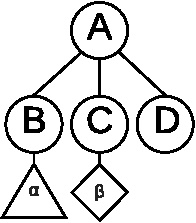
\includegraphics[scale=0.6]{img_ex/triangle.pdf}
% 		\caption{}
% 		\label{fig:triangle}
% 	\end{subfigure}%
% 	\hspace*{0cm}
% 	\begin{subfigure}[b]{0.30\textwidth}
% 		\raisebox{0mm}{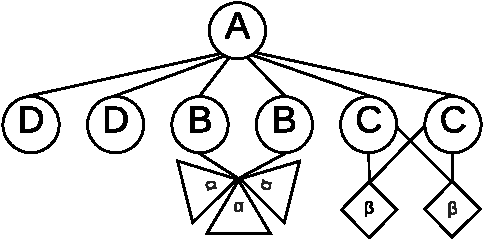
\includegraphics[scale=0.6]{img_ex/rep_triangle.pdf}}
% 		\caption{}
% 		\label{fig:rep_triangle}
% 	\end{subfigure}
% 	\vspace{-5mm}
% 	\caption{\small Subgraph Isomorphism. (a) pattern $R'$. (b) $\mathcal{R}$eplica$(R')$.}
% 	\label{fig:approx_motive}
% 	% \vspace{-5mm}
% \end{figure}
\subsection{Redundant Computations }
%First, we illustrate the source of redundant enumerations in the exact algorithm. %We now make an important
%observation: 
In many cases, to obtain a $\mathcal{R}$eplica, the identification of \emph{all}
instances of the query pattern may not be necessary. To illustrate, let us
revisit pattern $Q$ and $\mathcal{R}$eplica$(Q)$ in Figure ~\ref{fig:exact-EX}.
To obtain $\mathcal{R}$eplica$(R)$ for $Q$'s child $R$ via the exact approach,
edges $e_{1}=(v_{0}, v_{2})$ and $e_{2}=(v_{0}, v_{3})$ in $G$ are tried as
mappings for the \textit{extending edge} $(s_0, s_3)\in E_R$. To record $e_1$ as
a valid \textit{extension edge} mapping, we enumerate all instances of $R$ using
$\mathcal{R}$eplica$(Q)$ that are consistent with $(s_0,s_3)\mapsto e_1$. Now,
while considering the second edge $e_{2}=(v_{0}, v_{3})$ as a mapping of
$(s_0,s_3)$, the same enumeration scheme is exactly repeated. Here, we observe
that $e_2$ is \emph{symmetric} to $e_1$ since both of them share the extending
vertex $v_0$ and both $v_2$ and $v_3$ map to $s_3$. Consequently, any
instance mapping that is applicable for $e_1$ is likely to be
applicable for $e_2$. Thus, enumeration of \textit{all} instances as in
Algorithm \ref{algo:findallinstances} may be redundant. %
% We say high likelihood, because
%only in certain cases of homomorphism, this property may be violated and we
%discuss them in \S~\ref{sec:whyapprox}.
%if there extsists at least one edge $e=(V_0,V')$ in $E_G$, such that $V'\neq V_6$ and label of $V'$ is ``D'', we can conclude that  any instance 
%After all instances of $R$ with $e_{1}$ have been
%enumerated, the algorithm then begins to mine all instances containing $e_{2}$ in the
%following iteration. However, successfully enumerating even one instance with
%$e_{2}$ (out of the four possible) would suffice to record $e_{2}$ in
%$\mathcal{R}eplica(R)$ and consequently construct $\mathcal{R}eplica(R)$
%completely, since all other edges constituting the other three instances would
%have already been recorded in $\mathcal{R}$eplica$(R)$ during instances mining
%with $e_{1}$, in the previous iteration\footnote{{\footnotesize In fact, even
%while enumerating instances including $e_{1}$, mining any three of the four
%possible instances would have sufficed.}}. 

The impact of redundant computations in symmetric extensions can be further
appreciated from the example presented in Fig. \ref{fig:approx_motive}. 
\begin{figure}[t]
	\vspace{-2mm}
	\centering
	\hspace*{0.25cm}
	\begin{subfigure}[b]{0.12\textwidth}
		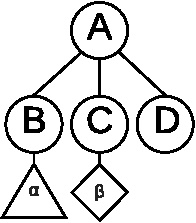
\includegraphics[scale=0.4]{img_ex/triangle.pdf}
		\caption{}
		\label{fig:triangle}
	\end{subfigure}%
	\hspace*{0cm}
	\begin{subfigure}[b]{0.30\textwidth}
		\raisebox{0mm}{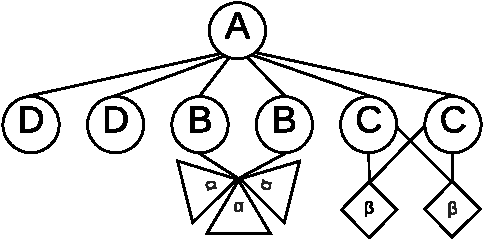
\includegraphics[scale=0.4]{img_ex/rep_triangle.pdf}}
		\caption{}
		\label{fig:rep_triangle}
	\end{subfigure}
	\caption{Subgraph Isomorphism. (a) pattern $R'$. (b) $\mathcal{R}$eplica$(R')$.}
	\label{fig:approx_motive}
	 \vspace{-0.10in}
\end{figure}
In Fig.
\ref{fig:approx_motive}, $R'$ is a subgraph pattern and we are again considering
an $(``A'',``D'')$ extension. However, unlike Fig. \ref{fig:exact-EX}, where
$``B''$ and $``C''$ are leaf nodes, here two arbitrary subgraphs $\alpha$ and
$\beta$ are attached. To obtain $\mathcal{R}$eplica$(R')$, the exact algorithm
would enumerate every instance of $R'$, which means the same three mappings of
$\alpha$ in $\mathcal{R}$eplica$(R')$ would be visited multiple times through
each $``B''$ for the two $(``A'',``D'')$ mappings; worse, for each $\alpha$,
both the mappings of $\beta$ would be enumerated twice - once through each
$``C''$. %The inefficiency due to repeated traversals becomes quite clear.
Clearly, these redundant computations can be avoided if we have the ability to
identify symmetric edges in the replica. For instance, the two $(``A'',``D'')$
edges in $\mathcal{R}$eplica($R'$) are symmetric and hence while considering the
second $(``A'',``D'')$ edge, we can simply re-use the instance enumerations of
the first $(``A'',``D'')$. Even more importantly, while enumerating the
instances corresponding to the first $(``A'',``D'')$ edge, we can observe that
the two $(``B'',\alpha)$ edges are symmetric and therefore enumerating the three
$\alpha$ subgraphs twice can be avoided by reusing the instance mappings from
the first $(``B'',\alpha)$ edge. The same applies to the $(``C'',\beta)$ edges
as well.%are also symmetric, and can be further used to reduce the computation

%The above examples highlight that symmetric extensions allow us a scope to re-use information from previous enumerations and drastically reduce the computation cost. 
Armed with this intuition, our goal, therefore, is as follows: ({\bf 1}) Identify if two edges in a replica are symmetric to each other, ({\bf 2}) For a group of symmetric edges, enumerate all instance mappings for only one edge from the group and then re-use the mappings for the remaining symmetric edges.
% instead of enumerating all instances from scratch, simply re-use the instances that were identified in the previously enumerated symmetric extension. %The next section details our algorithm to achieve this goal.


\begin{comment}
"exploring" the same mappings of
$\alpha$ and $\beta$ several times.  
 add ${(V_{0}, V_{7})}$ in $E(\mathcal{R}eplica(R))$ we require mining
only one instance of $R$. This is as 
to match a vertex $v\in V(G)$ and appropriate edges incident to $v$ in
$V(replica(R))$  and $E(replica(R))$ respectively for a pattern $R$, the
identification of \textit{all} instances of $R$ containing $v$ might not be
necessary. In other words, by identifying more instances containing $v$ than
might be necessary, we do not gain any additional information about the
\textit{replica} graph structure. This suggests that repeated traversals on
vertices during the course of identifying instances can perhaps be reduced
without losing structural information about the \textit{replica}.
\end{comment}
\vspace{-0.05in}
\subsection{Algorithm}
\label{sec:approxalgo}
First, we define when two edges in a replica are \emph{symmetric}.
\begin{defn}[Symmetric Edges]
Edges $e_1=(v_a,v_b)$ and $e_2=(v_c,v_d)$ in the replica are symmetric %be two edges from the data graph that are being considered as candidate extensions for the replica. $e_1$ and $e_2$ are symmetric 
if ({\bf 1}) $a=c$, and  ({\bf 2}) both $v_b$ and $v_d$ are mapped to the same node in the subgraph pattern.%, i.e. $L(V_b)=L(V_d)$, and $L(e_1)=L(e_2)$.
\end{defn}

%Algorithm \ref{algo:approx-instances} describes the approximate version of Algorithm \ref{algo:findallinstances}. 
We now describe the approximate algorithm in place of the exact version (Algorithm \ref{algo:findallinstances}). Recall, that edges in the replica are processed in the {\sf DFS} order. While processing edges in this order, we check
if it is symmetric to one of the already enumerated edges. If not,
the algorithm proceeds in exactly the same manner as in the exact version except
one difference: all of the successful mappings of a replica edge (or node) are
stored.  On the other hand, if the extension is symmetric, we do
not recompute from scratch. Rather, we reuse the mappings that were identified
in the previously enumerated symmetric edge, and among these mappings, we check
if there exists at least one instance to which the candidate edge for extension
can be mapped to. If one such instance is found, the candidate edge is added to the replica. %and all mappings from the previously enumerated symmetric edge are assumed to apply to the current edge as well.

%latest example for approximate:
\begin{figure}
\vspace{-0.20in}
	\begin{subfigure}[b]{0.5\textwidth}
		\centering
		% 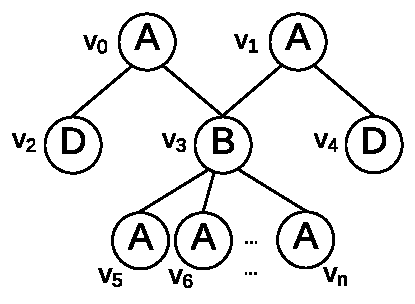
\includegraphics[scale=0.6]{img_ex/approxG.pdf}\hspace*{2.5em}
		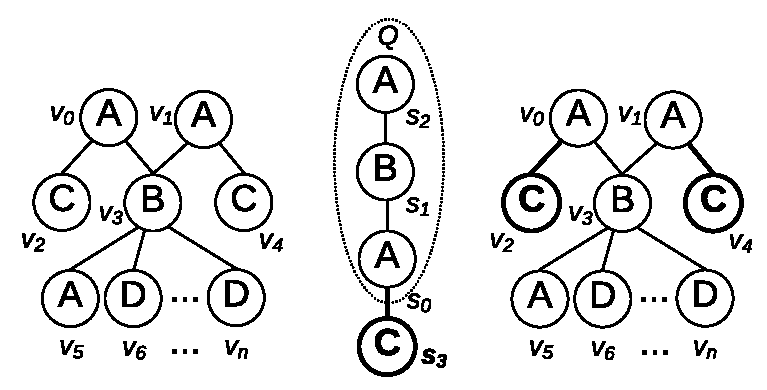
\includegraphics[scale=0.4]{img_ex/approx-new.pdf}\hspace*{2.5em}
		\caption{data graph $G$ (b) pattern $Q$ and extension to $R$ (c)
		Extending $\mathcal{R}$eplica$(Q)$ to $\mathcal{R}$eplica$(R)$}%
		\label{fig:exactq}
	\end{subfigure}%
	% \hspace*{\fill}
    % \begin{subfigure}[b]{0.15\textwidth}
    %         % \centering
    %         \hspace{4mm}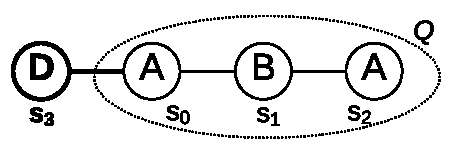
\includegraphics[scale=0.6]{img_ex/approxR.pdf}
    %         \caption{Parent $Q$}
	% 		\label{fig:exactq}
    % \end{subfigure}%
    % \hspace*{\fill}
    % % \captionsetup[subfigure]{labelfont=bf,textfont=normalfont,singlelinecheck=on,justification=raggedright, skip=-5pt}
	% \begin{subfigure}[b]{0.2\textwidth}
    %         % \centering
    %         \hspace{-2.5mm}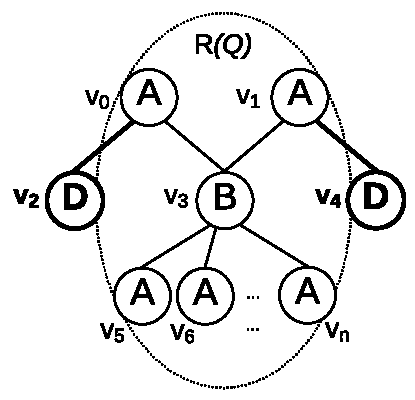
\includegraphics[scale=0.6]{img_ex/approxrepR.pdf}
    %         \vspace{-4.5mm}
    %         \caption{$\mathcal{R}$eplica$(Q)$}
	% 		\label{fig:exactrepq}
	% \end{subfigure}
	% % \captionsetup[subfigure]{skip=-2pt}
	% \begin{subfigure}[b]{0.15\textwidth}
	% 	% \centering
	% 	\hspace{4mm}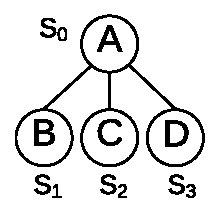
\includegraphics[scale=0.6]{img_ex/patternR.pdf}
	% 	\caption{Child $R$}
	% 	\label{fig:exactr}
	% \end{subfigure}%
	% \hspace*{\fill}
	% \begin{subfigure}[b]{0.3\textwidth}
	% 	% \centering
	% 	\hspace{0mm}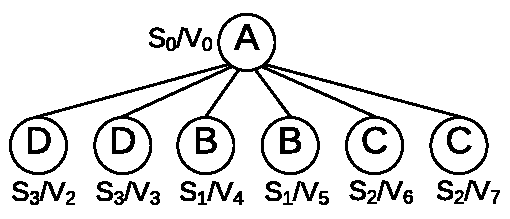
\includegraphics[scale=0.6]{img_ex/replicaR.pdf}
	% 	\vspace{-0.25mm}
	% 	% \vspace{-1.3\baselineskip} %not needed because figures are aligned
	% 	% naturally unline above case
	% 	\caption{$\mathcal{R}$eplica$(R)$}
	% 	\label{fig:exactrepr}
	% \end{subfigure}
	% \captionsetup[figure]{skip=200pt}
    % \vspace{-1.75\baselineskip}
	\caption{$\mathcal{R}$eplica generation for a new subgraph pattern}
	\label{fig:approxex}
	 \vspace{-0.05in}
\end{figure}
\vspace{-0.05in}
\begin{exple}
	Consider Fig. \ref{fig:approxex}, where edge $(s_0,s_3)$ is
	extended from pattern $Q$ to get child $R$. To obtain
	$\mathcal{R}$eplica$(R)$ from $\mathcal{R}$eplica$(Q)$, \textsc{CSM-A} first
	attempts to enumerate instances of $R$ in $G$ by mapping edge $(v_0, v_2)$ to $(s_0,s_3)$. Following this mapping, CSM-A, like CSM-E,
	enumerates all isomorphisms by mapping
	$(s_0,s_1)\mapsto(v_0,v_3)$ and $(s_1,s_2)\mapsto
	\{(v_3,v_5),(v_3,v_1)\}$. Thus, nodes
	$v_1$ and $v_5$ are considered valid mappings for $s_2$. Next, when
	\textsc{CSM-A} attempts to enumerate instances after mapping
	$(s_0,s_3)\mapsto(v_1, v_4)$, it recognizes the symmetric relation between
	$(v_1,v_3)$ and $(v_0,v_3)$ and thus only traverses the
	already-\emph{confirmed} mappings set $\{v_1,v_5\}$ instead of all the neighbors of $v_3$. Furthermore, even while traversing the set of confirmed mappings, we stop as soon as one instance is found, which further reduces the computation cost.  %until
%	it finds \emph{one} instance.%, and thereby avoiding redundant traversals
%	over already-explored vertices in $C_{v_3,s_2}$. In this particular example, 
%Consequently, instead of iterating over $|C_$ nodes, the approximate version processes only $1$ node for the symmetric edge.

	
	% Initially, $Q$ and $\mathcal{R}$eplica$(Q)$ are
	% shown in Figures \ref{fig:exactq}, \ref{fig:exactrepq}, respectively. Child
	% $R$, extended from $Q$ at \emph{extending node} $S_0$ using the
	% \emph{candidate edge} $(A, D)$ is given in Figure \ref{fig:exactr}. Assume
	% \emph{DFS List} starting at $S_0$ records edges $(S_0, S_1)$ and $(S_0,
	% S_2)$ in that order. To construct $\mathcal{R}$eplica$(R)$, the algorithm jumps to
	% $Mapping(S_0)$ in $\mathcal{R}$eplica$(Q)$, i.e. ${V_0}$, followed by ${V_1}$.
	% Assume, $(V_0, V_6), (V_0, V_7)\in E(G)$ map to $(A, D)$; but no such
	% mapping edges exist incident to $V_1$ in $G$. All instances of $R$ thus found
	% would result in $\mathcal{R}$eplica$(R)$ depicted in Figure \ref{fig:exactrepr}.
	% %
	\label{ex:approx}
	\end{exple}
\vspace{-0.05in}
\begin{comment}
to implement the idea of reducing repeated
traversals over "already-explored" vertices for accelerated $\mathcal{R}$eplica
construction. We attempt to avoid enumerating those instances during
construction that do not provide new information about the $\mathcal{R}$eplica,
as a strategy to reduce complexity. Before discussing this method,
we define three indices in addition to the mappings in \S~\ref{sec:rep_data}
that will be used to track enumeration:

\para{Potential children set ${(P_{v',c})}$}: (indexed for each $v'\in
V_{\mathcal{R}(Q)}$ matched to $p\in V_{Q}$ for each child $c\in children(p,Q)
\in V_{Q}$) Stores every vertex $w'\in V_{\mathcal{R}(Q)}$ such that $w'$ is a
candidate for matching $c$, given $v'$ is matched to $p$.

\para{Enumerated set $({E_u})$}: (indexed for each $u\in V_Q$) Stores every
vertex $w'\in V_{\mathcal{R}(Q)}$ that is matched to $u$ such that $\forall
c$ $\in children(u,Q)\ P_{w',c}=\emptyset$. In other words, $E_{u}$ stores all
mappings of vertex $u$ in $V_{\mathcal{R}(Q)}$ that have been
"fully-explored" for \emph{all} child mappings, as indicated by empty
Potential sets.

% $v$ has been fully-explored for all possible child mappings below it.
\para{Confirmed children set ${(C_{v',c})}$}: (indexed for each $v'\in
V_{\mathcal{R}(Q)}$ mapped to $p\in V(Q)$ for each child $c\in children(p,Q) \in
V_Q$) Stores every vertex $w'\in V_{\mathcal{R}(Q)}$ such that: (1) there
exists at least one instance containing $(p, v')$ and $(c,w')$, and
(2) $w'$ has been completely \emph{enumerated} for all its children, i.e. $w'\in E_{c}$.

% for the $\mathcal{R}$eplica data structure:
% for the \textit{replica}:
% However, the strategy also could miss identifying a few relevant instances in
% certain cases which could possibly result in the loss of some information
% about the \textit{replica} graph and its mappings lists (Section
% \ref{subsubsec:replica-ds}). Consequently, the \textit{replica} $R_a$ thus
% obtained would be an \textbf{approximation} of the complete \emph{replica}
% $R_c$ such that $V_{R_a} \subseteq V_{R_c}$ and $E_{R_a} \subseteq E_{R_c}$ .
% In Section \ref{sec:experiments}, we demonstrate empirically that such an
% approximation scheme, while enabling computational tractability, does not
% significantly affect quality of the top-\textit{k} results.
%!!!write that misses are insignificant as proved in the experiments write that
%!!!approximation means missing correct not including incorrect mappings
% Algorithm \ref{algo:approx-instances} describes this approximation scheme.
\end{comment}
\begin{comment}
\begin{algorithm}[t!]
{   \scriptsize
	% \SetAlgoLined
	% \DontPrintSemicolon
	\SetNoFillComment
	\caption{\textsc{FindAllInstancesApprox}}\label{algo:approx-instances}
	%\dontprintsemicolon
	% \nonl\textbf{Input:} $G$, parent $Q$, $replica(Q)$, child $R$, $DFS$ $List$
	% of $Q$, partial isomorphism of $R$: $instance$, $\mathbb{I}$ \textit{(initialized to
	% $\emptyset$)}\;
	\nonl \textbf{Input:} data graph $G=(V,E,L)$, parent
	pattern $Q=(V_Q,E_Q,$ $L)$, $\mathcal{R}$eplica$(Q)=(V_{\mathcal{R}(Q)}$,
	$E_{\mathcal{R}(Q)}$, $L)$, child pattern $R=(V_R$, $E_R$, $L)$,
	   $DFS\ List(Q)$, partial isomorphism of $R$: $instance$, $\mathbb{I}$\;
   \nonl \textbf{Output:} $\mathbb{I}: $ set of all relevant instances of $R$ in $G$ consistent with input partial isomorphism $instance$\;   
	% \nonl \textbf{Output:} set of relevant instances $\mathbb{I}$ of $R$ in $G$
	% consistent with input partial isomorphism $instance$\;
	\vspace{0.3mm}\;
	\uIf {$instance$ \textup{is} {\sf Found}}
	{
		% Update $E_{l'}$ for each  $l'\in Leaves(Q)$\; 
		% $\forall l\in Leaves(Q)\ E_{l}\leftarrow E_{l} \cup \{instance(l)\}$ \;
		\textbf{return} $\{instance\}$\;
	}
	\Else
	{
	$e(p,c) \leftarrow$
		\textsc{NextQueryEdge($DFS\ List(Q)$)}\; 
		% \nonl ~ \tcp*[h]{$[[e(p,c) \in E(Q)\wedge c
		% \in children(p)]]$}\; 
		$v'\leftarrow$ $instance(p)$\; 
		% \textbf{boolean} $InstanceFound$\; 
		% \nonl $[[\ v\in V(replica(Q))\wedge (p,v)\in instance]]$\;
		\uIf{$e$ \textup{is a} {\sf backward edge}}
		{
			\uIf{\textup{an edge} $(v',instance(c))$ \textup{exists in} $E_{\mathcal{R}(Q)}$}
			{
				$\mathbb{I} \leftarrow \mathbb{I}\ \cup$ \textsc{FindAllInstancesApprox({$G$}, $Q$, $\mathcal{R}eplica(Q)$, $R$, $DFS\ List(Q)$, $instance$, $\mathbb{I}$)}\;
			}
			\Else{\Return $\emptyset$}
		}
		% (\tcp*[h]{{$e$ is a forward edge}})
		\Else{
	\uIf(\tcp*[f]{one-time}){${P_{v',c}}$ \textup{does not already exist}}
	{${P_{v',c}}\leftarrow$ \textsc{FilterCandidates($v'$, $c$, $Q$, $\mathcal{R}eplica(Q)$)\;}
		${C_{v',c}}\leftarrow \emptyset$\;% \tcp*[f]{initialization}\;
		\ForEach {$w' \in P_{v',c}$ \textup{such that $w'$ is not matched}}{ 
			$instance.{\sf add}(c\mapsto w')$\;
		$\mathbb{I'} \leftarrow $
		\textsc{FindAllInstancesApprox($G$, $Q$, $\mathcal{R}eplica(Q)$, $R$, $DFS\
		List(Q)$, $instance$, $\mathbb{I}$)} \;
			\uIf {$\mathbb{I'} \neq \emptyset$}
			{
			%$InstanceFound\leftarrow {\sf True}$\; 
			$\mathbb{I}\leftarrow \mathbb{I}\cup\mathbb{I'}$\;
			\makebox[\linewidth][l]
			{\hspace{-0.8mm} $P_{v'\hspace{-0.5mm},c}\Arrow{0.2cm}\ P_{v'\hspace{-0.5mm},c}\backslash\{\hspace{-0.3mm}w'\hspace{-0.3mm}\}$ \hspace{-0.5mm}and
				$C_{v'\hspace{-0.5mm},c}\Arrow{0.2cm}\ C_{v'\hspace{-0.5mm},c}\hspace{-0.6mm}\cup \hspace{-0.6mm}\{\hspace{-0.3mm}w'\hspace{-0.3mm}\}$\;}} 
				$instance.{\sf delete}(c\mapsto w')$\;}
	}
	\Else{
		\ForEach{$w' \in C_{v',c}$ \textup{such that $w'$ is not matched}} 
		{			$instance.{\sf add}(c\mapsto w')$\; 
		$\mathbb{I'} \leftarrow $ \textsc{FindAllInstancesApprox($G$, $Q$, $\mathcal{R}eplica(Q)$, $R$, $DFS\
		List(Q)$, $instance$, $\mathbb{I}$)} \;
			\makebox[\linewidth][l]{\lIf {$\mathbb{I'} \neq \emptyset$}
		{$\mathbb{I}\Arrow{0.28cm}\ \mathbb{I}\cup\mathbb{I'}$ and \textbf{break}\;}}
		$instance.{\sf delete}(c\mapsto w')$\;
		}
	% \lIf{$\ \forall s \in children(p)\ P_{v',s} = \emptyset$}
	% { $E_{p} \leftarrow E_{p} \cup \{v'\}$\;} 
	}
	}
	\Return{$\mathbb{I}$}\;
	}}
\end{algorithm}
\end{comment}
\begin{comment}
Algorithm \textsc{FindAllInstancesApprox} is a modification of Subroutine
\ref{algo:getreplica_}.1. (\textbf{1}) In the general case (lines 5-23), the
algorithm begins by invoking \textsc{NextQueryEdge} which returns $e(p,c)\in
E_Q$ similar to Subroutine \ref{algo:getreplica_}.1. Thus, $c$ is to be matched
in the current iteration. The algorithm then checks for the existence of the
Potential children set for storing candidate vertices for matching $c$, given
that $p$ is mapped to $v'$. If this set $P_{v',c}$ does not exist, it is
initialized by invoking \textsc{FilterCandidates} which stores all candidates
$w'\in V_{\mathcal{R}(Q)}$ (\S \ref{??}). Note that unlike in Subroutine
\ref{algo:getreplica_}.1, the candidates set $P_{v',c}$ is constructed only once
and indexed so that in the event of any subsequent visit(s) to $v'$, only the
candidates remaining in $P_{v',c}$ are attempted for matching $c$. Similarly,
confirmed children set $C_{v',c}$ is initialized once as an empty set and
indexed.
% \begin{comment}
% Thus, set $P_{v,c}$ is constructed once when a
% match for $c$ is being sought for the first time with $p$ having been mapped to
% $v$, and indexed. Similarly, confirmed children set $C_{v,c}$ is initialized as
% an empty set and indexed. In the event of any subsequent visit, the algorithm
% simply considers candidates remaining in $P_{v,c}$ for matching $c$.
% is a recursive algorithm. In the general
% (recursive) case (lines??-??), it begins by invoking \textsc{NextQueryEdge}
% which returns one edge at a time from $E(Q)$ in the order of the rooted $DFS\
% List$. Edge $e(p,c)$ thus returned connects vertices $p,c \in V(Q)$ such that
% $c\in children(p)$ as per the $DFS\ List$ and $c$ is the pattern vertex to be
% matched next ($p$ is matched to $v \in V(replica(Q))$). The algorithm then
% checks for the existence of the potential children set for storing candidate
% vertices for matching $c$, given that $p$ is mapped to $v$. If this set
% $P_{v,c}(\subseteq V(replica(Q)))$ does not exist, it is computed by invoking
% \textsc{FilterCandidates} which stores all vertices $w\in V(replica(Q))$ such
% that: (1) $w$ is contained in the \textit{replica} adjacency list of $v$; (2)
% $c$ exists in the inverse mapping list of $w$. That is, $\forall$ $w \in
% P_{v,c}$, $c\in InverseMap(w)$; (3) The edge label of $(v,w)\in E(replica(Q))$
% matches that of $(p,c)\in E(Q)$. Thus, set $P_{v,c}$ is constructed once when a
% match for $c$ is being sought for the first time with $p$ having been mapped to
% $v$, and indexed. Similarly, confirmed children set $C_{v,c}$ is initialized as
% an empty set and indexed. In the event of any subsequent visit, the algorithm
% simply considers candidates remaining in $P_{v,c}$ for matching $c$.
% \end{comment} 
(\textbf{2}) Next, for each unmatched $w'\in P_{v',c}$, the algorithm attempts a
matching for $c$ followed by a recursive invocation for matching remaining
vertices following the \emph{DFS List} of $Q$'s edges, similar to Subroutine
\ref{algo:getreplica_}.1. A boolean \emph{InstanceFound} is set to {\sf True} if
it finds at least one instance including $(c,w')$ for some $w'\in P_{v',c}$
during the recursive call, and set of all found instances is appended to
$\mathbb{I}$. During the recursive call, if a $w'$ gets inserted into the
Enumerated set for $c$ (i.e. $E_c$) and an instance is found containing
$(c,w')$, $w'$ is transferred from $P_{v',c}$ to $C_{v',c}$: the intuition is
that since $w'\in E_c$, candidates for matching vertices in $children(c, Q)$ at
$w'$ have been fully explored and an instance existence demonstrates that none
of these candidate sets could have been empty to begin with, thus, $w'$ can be
added to Confirmed children set $C_{v',c}$. Therefore, $C_{v',c}$ stores all
such explored vertices $w'$ such that subsequent traversals over $w'$ as a
mapping of $c$ after $v'$ could be avoided to reduce repeated traversals.
Vertices in $P_{v',c}$ move to $C_{v',c}$ as and when they get \emph{fully}
explored, leaving only the remainder in $P_{v',c}$ for explorations in
subsequent visits to $v'$. (\textbf{3}) Suppose, the algorithm fails to find any
instance even after considering every $w'\in P_{v',c}$. (A possible
scenario where this could happen is if $P_{v',c}=\emptyset$, after all original
candidates have been confirmed and transferred to $C_{v',c}$). In such a
scenario, \emph{InstanceFound} would remain {\sf False} after the first loop.
The algorithm would then start iterating over $C_{v',c}$, the set of confirmed
children but only till one instance is found including some $w' \in
C_{v',c}$, and \emph{InstanceFound} is set to {\sf True}. This is as all vertices in
$C_{v',c}$ have already been fully explored, thus only as many confirmed $w'$
should be chosen for attempted matching as required until an instance is found.
% Completely avoiding traversal over $C_{v',c}$ would have resulted in failure to record many relevant instances. 
(\textbf{4}) Finally, for every $s\in children(p, Q)$ if the candidates
set $P_{v',s}$ is exhausted, $v'$ is appended to $E_{p}$. This means that
\textit{all} candidate child mappings possible with $v'$ matched to $p$ have
been traversed and confirmed. The \textit{General Case} returns with the set of
all instances mined that were determined to be "relevant" for obtaining
$\mathcal{R}$eplica structural information.

% any subsequent exploration
% of $w'$ as a mapping of $c$ from 
% for
% every vertex $w \in P_{v,c}$ such that $w$ has not already been mapped to some
% other pattern vertex in the current $instance$, the algorithm attempts the
% mapping $(c,w)$ in $instance$ and recursively calls
% \textsc{FindAllInstancesApprox} to match remaining pattern vertices following
% the $DFS\ List$ of edges. It sets a boolean $InstanceFound$ to $True$ if it
% finds at least one $instance$ in the recursive call and appends the set of all
% found instances to $\mathbb{I}$. During the recursive call, if $w$ gets inserted
% into the enumerated set for $c$ ($E_c$), it is transferred from $P_{v,c}$ to
% $C_{v,c}$. Finally, $(c,w)$ is removed from $instance$ and the next valid
% candidate in $P_{v,c}$ tried as a possible matching for $c$ in the following
% iteration. Suppose, the algorithm fails to find any $instance$ even after
% considering every $w\in P_{v,c}$. (A possible scenario where this could happen
% is if $P_{v,c}=\emptyset$, after all original candidates have been confirmed and
% transferred to $C_{v,c}$). In such a scenario, $InstanceFound$ would remain
% false after the first loop. The algorithm would then start iterating over
% $C_{v,c}$, the set of confirmed children till the time an $instance$ is found
% for some $w' \in C_{v,u}$ and $InstanceFound$ is set to $True$. Finally, if the
% candidates set $P_{v,c'}$ for \textbf{every} $c'\in children(p)$ is exhausted,
% $v$ is appended to the enumerated set for $p (E_{p})$. This means that
% \textit{all} possible candidate child mappings have been traversed and
% confirmed. Note that in lines ??-??, child mapping $w$ if inserted into $E_{c}$
% gets tranferred from $P_{v,c}$ to $C_{v,c}$. This is because any subsequent
% searches for possible mappings of $c$ at $v$ can ignore all $w' \in C_{v,c}$
% since such a $w'$ has been completely "enumerated" and thus matching it to $c$
% would result in repeated traversals over already explored portions of the graph.
(\textbf{5}) The base case (lines 1-3) hits when the algorithm finds an
instance of the child pattern $R$ (i.e., $|instance|=|V(R)|$). The algorithm
records the mappings of every $l\in Leaves(Q)$ in the corresponding enumerated
sets $E_{l}$ since $children(l,Q)=\emptyset$ and thus there cannot exist any child
mappings. Note that this means that mappings of all leaves belonging in relevant
Potential sets immediately transfer to the corresponding Confirmed sets upon
discovery of the instance. Finally, an \emph{instance} is returned. This
completes the algorithm. 
\textcolor{red}{\\comment AP: reader should have answers to these at this point:
1. what is the idea behind defining an "enumerated" set of vertices\\
2. why confirmed set need not be traversed, only P set should (it's the whole point of
confirmed set)\\
3. why should "C" set be traversed only if no match in "P" that too only until one
instance found\\
4. why does a child vertex have to be in Enumerated AND one instance found, to
be put into confrrmed set\\
}

\textcolor{red}{cut down on example text}
As an example to understand Algorithm \ref{algo:approx-instances}, consider the
$\mathcal{R}$eplica construction example in Fig. \ref{fig:exactex}. Starting at
$V_{0}$ as a match for $A\ (S_{0})$, $D\ (S_{3})$ is matched to $\{V_6, V_7\}$.
First, with $V_6$, set $P_{V_{0},S_{1}}$ is initialized to $\{V_2,V_3\}$, the
candidates for matching $B\ (S_{1})$. Choosing $V_2$ for this matching, the
candidates set for matching $C\ (S_2)$, $P_{V_0,S_2}$ is initialized to $\{V_4,
V_5\}$. Matching both these vertices results in an instance each, corresponding
to which $V_4$ and $V_5$ are inserted in $E_{S_2}$ and $V_2$ in $E_{S_1}$, since
$S_1, S_2\in Leaves(Q)$. $V_4$ and $V_5$, belonging in $E_2$, are transferred
from $P_{V_0, S_2}$ to $C_{V_0, S_2}$. Similarly, $V_2$ to $C_{V_0,S_1}$ from
$P_{V_0,S_1}$. Next, $V_3$ from $P_{V_0,S_1}$ is attempted for matching $S_1$,
and recursion is invoked for matching $S_2$. However, now $P_{V_0,S_2}$ is
empty, thus, the algorithm starts iterating over confirmed vertices in
$C_{V_0,S_2}$ until it finds an instance. It does so with $V_4$ which results in
the third instance being mined and $V_3$ also moving to $C_{V_0,S_1}$. This
completes the search with $D$ matched to $V_6$. Note that a fourth possible
instance using $V_5$ is not enumerated with \textbf{no loss} in $\mathcal{R}$eplica
information. Similarly, now with $(D,V_7)$ in \textit{instance}, set
$P_{V_0,S_1}$ is empty for matching $B$. Therefore, vertices in
$C_{V_0,S_1}=\{V_2, V_3\}$ are tried until an instance is found: choosing $V_2$,
we again encounter an empty $P_{V_0,S_2}$ for matching $C$ and once again
$V_4\in C_{V_0,S_2}$ is matched. Since this results in an instance, $V_6$ is
recorded in $\mathcal{R}$eplica. Moreover, $InstanceFound$ is set to {\sf True}
for both $B$ and $C$ and thus the search terminates. Thus, making use of the
additional indices, Algorithm \ref{algo:approx-instances} could obtain
\textbf{exact} $\mathcal{R}$eplica$(R)$ after mining just four instances, out of total eight
possible.
\end{comment}
\begin{comment}
\textcolor{red}{comment AP: 1. in the intro (also), we should make it clear that
CSM-A is the primary CSM approach, not CSM-E\\
2. also, need to make it clear somehwere CSM-E =
algo\ref{algo:getreplica}+\ref{algo:findallinstances}, corr. comp.\\
CSM-A = algo\ref{algo:getreplica}+\ref{algo:approx-instances}, corr. comp.}
\end{comment}
\vspace{-0.05in}
\subsection{Properties} 
%In this section, we
%establish two key properties of Algorithm~\ref{algo:approx-instances}.
% \subsubsection{Why is this an approximation?} 
% \label{sec:whyapprox}
%\textcolor{blue}{Firstly, Algorithm \ref{algo:getreplica} in conjunction with
%\ref{algo:approx-instances} can fail to identify some relevant instances in
%certain cases, resulting in partial loss of information about the
%$\mathcal{R}$eplica. In 
To understand the \emph{approximation} in the above algorithm, let us revisit
Example~\ref{ex:approx}. %While matching edge $(s_0,s_3)\mapsto (v_0,v_2)$,
%\textsc{CSM-A} identifies nodes $v_1$ and $v_3$ as valid mappings for $s_2$. 
The symmetric extension $(v_1,v_4)$ searches only within the confirmed mappings
$v_1$ and $v_5$ to match $s_2$. However, $s_2$ can also be mapped to $v_0$ to constitute an instance with $s_0\mapsto v_1$, $s_3\mapsto v_4$ and $s_1\mapsto v_3$, % $(v_1,v_3)$ is mapped to
%(s_0,s_1)$ and $(v_1,v_3)$ mapped to $(v_1,v_3)$, then $v_0$ is a valid mapping for $s_3$
 which CSM-A will fail to enumerate. To
generalize, CSM-A may miss a mapping if some node in the data graph can be
mapped to multiple nodes of the subgraph pattern. In Fig.~\ref{fig:approxex},
this occurs, where $v_0$ (or $v_1$) may be mapped to either $s_2$ or $s_0$. It
can be guaranteed, however, that there are no false positives since any edge
that we add to the replica, corresponds to at least one instance from the
subgraph. Consequently, we can state the following.

%after matching the symmetric edge $(v_1,v_3)$ with $(s_0,s_1)$ would fail to
%consider a possible isomorphism with $(s_1,s_2)\mapsto (v_3,v_0)$. As a result
%$v_0$ would not be recorded in \textit{Mappings} index for $s_2\in
%V_{\mathcal{R}(R)}$ (similarly $s_2$ would not be present in associated
%\textit{Mappings$^{-1}$}).}
%The second property we present as a theorem:
\begin{lma}
	\label{lem:lowerbound}
	For any pair of subgraphs $Q,R\in T$, consider $\sigma(Q)$ to be the {\sf
	MNI-support} and $\kappa(Q,R,h)$ the correlation value between $Q$ and $R$
	at $h$-hop separation computed via \textsc{CSM-A}, and $\sigma^*(Q)$,
	$\kappa^*(Q,R,h)$ be the respective values computed via \textsc{CSM-E}. Then:
	(1) $\sigma(Q)\leq \sigma^*(Q)$, and (2) $\kappa(Q,R,h) \leq \kappa^*(Q,R,h)$.
	% $\sigma^*(R)$ the exact support computed after \textsc{CSM-E}. 
\end{lma}

\textsc{Proof:} The support and correlations counts obtained through CSM-A is a lower bound to CSM-E %The upper-bounds in Lemma \ref{lemma:sec4} exist because 
since {\sf CSM-A} does not return any false positives during instances enumeration. In other words, the set
of pattern instances enumerated in {\sf CSM-A} is always a subset of the
(exhaustive) set found by {\sf CSM-E}. $\hfill\square$ %Thus, frequency computed after
%approximate $\mathcal{R}$eplica construction can never exceed the true
%value. For the same reason, $\kappa$ values are also bounded by the true values. 
\begin{comment}
In \S~\ref{sec:experiments}, empirical analyses on performance
demonstrate the significant computational efficiency offered by the approximate
method in performing (approximate) subgraph isomorphism. This approach is used in 
fast computing the $\mathcal{R}$eplica, as well as for correlation
computation (\S~\ref{sec:cor_compute}) while having minimal to almost no
impact on top-$k$ result quality, as characterized by the Kendall's Tau coefficient
among other metrics. {\sf CSM-A} approach makes the $\mathcal{R}$eplica generation  
problem tractable on large (and dense) graphs, where even {\sf CSM-E} fails \st{thus
we present CSM-A as our primary contribution for correlated subgraphs mining.}
\end{comment}
% \begin{theorem}
% Lower bound
% \end{theorem}
%  \textsc{FindAllInstancesApprox}, 
% \begin{exple}
% 	For input graph $G$ and graph pattern $Q_1$ in Figure~\ref{fig:correlation},
% 	the instances are
% 	given by $\mathbb{I}=\{u_1u_3,u_2u_3,u_7u_3,u_7u_6\}$. However, its MNI support is two, since
% 	node $v_2$ has only two corresponding images: $u_3$ and $u_6$. Thus, we group the instances
% 	according to the presence of $u_3$ and $u_6$ as follows: $\mathbb{I'}=\{u_1u_2u_7u_3,u_7u_6\}$.
% \end{exple}
